% TEMPLATE for Usenix papers, specifically to meet requirements of
%  USENIX '05
% originally a template for producing IEEE-format articles using LaTeX.
%   written by Matthew Ward, CS Department, Worcester Polytechnic Institute.
% adapted by David Beazley for his excellent SWIG paper in Proceedings,
%   Tcl 96
% turned into a smartass generic template by De Clarke, with thanks to
%   both the above pioneers
% use at your own risk.  Complaints to /dev/null.
% make it two column with no page numbering, default is 10 point

% Munged by Fred Douglis <douglis@research.att.com> 10/97 to separate
% the .sty file from the LaTeX source template, so that people can
% more easily include the .sty file into an existing document.  Also
% changed to more closely follow the style guidelines as represented
% by the Word sample file. 

% Note that since 2010, USENIX does not require endnotes. If you want
% foot of page notes, don't include the endnotes package in the 
% usepackage command, below.

% This version uses the latex2e styles, not the very ancient 2.09 stuff.

% Updated July 2018: Text block size changed from 6.5" to 7"

\documentclass[letterpaper,twocolumn,10pt]{article}
\usepackage{usenix2019,epsfig,endnotes}

\begin{document}

%don't want date printed
\date{}

%make title bold and 14 pt font (Latex default is non-bold, 16 pt)
\title{\Large \bf HGFRR: Hidden Geographical Fractal Random Ring}

%for single author (just remove % characters)
%\author{
%{\rm Your N.\ Here}\\
%Your Institution
%\and
%{\rm Second Name}\\
%Second Institution
% copy the following lines to add more authors
% \and
% {\rm Name}\\
%Name Institution
%} % end author

\author{
{\rm Anonymous Authors}\\
}

\maketitle

% Use the following at camera-ready time to suppress page numbers.
% Comment it out when you first submit the paper for review.
\thispagestyle{empty}

\subsection*{Abstract}
This is the abstract.

\section{Introduction}
% Flow:
%
% start from talking about current blockchain systems, transaction rate is getting increasing
% ->
% problem is: current blockchain systems are based on kademlia (dht) structure, which is efficient on node discovery and data look up, however, broadcast suffers traffic congesion and inefficient convergence (gossip)
% ->
% many improvements are made on gossip, not quite efficient, still suffers bandwidth problem
% ->
% less p2p network are designed for blockchain, talk about p2p networks in other domains
% ->
% analysis blockchain needs and those p2p networks does not fit\\
% ->
% moreover, current blockchain systems didn't address geographical feature
% ->
% moreover, current blockchain systems didn't address security problem from the p2p layer
% ->
% talk about hgfrr, give a overview, analysis result, implementation overview, evaluation result
% ->
% summarize our feature \& contributions
% ->
% paper structure overview

A blockchain is essentially a distributed ledger that permanently records the transactions among parties \cite{iansiti2018truth}. The transactions recorded are verifiable and resistant to modification without the need of a centralized third party. The decentralization nature and proved immutability have led to the emergence of cryptocurrencies which leverages the blockchain system as their cornerstone, the most salient example being Bitcoin \cite{nakamoto2008bitcoin}. Blockchain systems are based on consensus protocols to achieve chain consistency. With tremendous works focused on consensus layer to increase the blockchain system efficiency and transaction rate, broadcast frequency is growing.

%Despite the popularity of cryptocurrencies, general and all-purpose blockchain systems that accommodate various applications, such as Ethereum \cite{wood2014ethereum} have been proposed. However, although Ethereum is a Turing-complete system \cite{wood2014ethereum}, it is in essence designed for the cryptocurrency based on it. Hence the Proof-of-Work (PoW) consensus has been utilized used to support the valuation of the cryptocurrency in the socioeconomic sense, which results in poor efficiency. To facilitate general-purpose applications in a more efficient manner, other consensus protocols have been proposed to improve the performance of the blockchain systems in different scenarios such as Proof-of-Stake \cite{kiayias2017ouroboros}, Proof-of-Luck \cite{milutinovic2016proof}, and Proof-of-Membership \cite{kogias2016enhancing}. Hyperledger Sawtooth \cite{sawtooth} utilizes Intel Software Guard eXtentions (SGX, introduced below) to trust nodes and proposes Proof-of-Elapsed Time believed to be highly efficient. Additionally, EOS \cite{eosio} based on DPoS, NEO \cite{hoxha2018hashgraph} based on DBFT, and Hyperledger Fabric \cite{cachin2016architecture} are all examples of new blockchain systems which are claimed to achieve more than 10k transaction rate \cite{bach2018comparative}.

Unfortunately, experiments and studies \cite{cachin2016architecture, xueos, li2018scaling} already show that the network layer became the bottleneck of further growing of transaction rate. For example, EOS report \cite{xueos} shows that EOS is sensitive to network latency. Higher network latency caused by other bandwidth-intensive applications in the same network or high client transaction input rate can lead to significant drop of throughput. Hyperledger Fabric \cite{cachin2016architecture} also shows that its throughput is capped by the low efficiency of the P2P network. However, current blockchain systems are based on Distributed Hash Table (DHT) structure and message broadcast in a Gossip manner \cite{eugster2004epidemic}. It is efficient in terms of node discovery and data look up. 

However, broadcasting messages suffers from traffic congestion and inefficient convergence problems when transaction rate gets higher. Our key insight is that the Gossip algorithm used to broadcast a message does not fit in the demand for P2P networks from blockchain systems. Although many improvements has been made on Gossip algorithm such as adding unique message ID, using Time-to-Live field to control flooding, using pull-version sending mechanism to reduce repeated messages, our evaluations show that they are not efficient, and still suffer from traffic congestion problem. 

% Blockchain systems' requirements are different from other Peer-to-Peer applications: (i) on-demand streaming allows users to look up data in the P2P network and download stream data from the source, e.g. BitTorrent-based streaming systems like BASS \cite{dana2005bass}, Peer-Assisted \cite{carlsson2007peer}, LiveBT \cite{lv2007livebt}, and Give-To-Get \cite{mol2008give}; (ii) audio/video conferencing applications deal with small scale point-to-point connected networks which requires low latency, e.g. Skype \cite{baset2004analysis}; (iii) peer-to-peer file sharing makes efficient indexing and searching possible, e.g. Napster \cite{saroiu2003measuring}, Gnutella \cite{ripeanu2001peer}, and KaZaA \cite{good2003usability}; (iv) video streaming applications enables single-source broadcasting efficient, e.g. SplitStream \cite{castro2003splitstream}, Bullet \cite{kostic2003bullet}, and ChainSaw \cite{pai2005chainsaw}. (i) and (ii) are not relevant to the context of blockchain systems since nodes in a blockchain system network should be in a large scale and broadcasting a message is an active operation instead of searching and downloading data. (iii) and (iv) are more similar to blockchain systems' use case. However, P2P file sharing is not real-time and the broadcast model in a blockchain system is not indexing and searching. In video streaming, time is stringent and the network size can be large-scale. However, it is a data or bandwidth-intensive communication which means control messages in a broadcast operation are relatively small compared to the data to transmit.

Blockchain systems require two main functions from the underlying P2P network from : peer discovery and message dissemination. For peer discovery, DHT-based protocols such as Chord \cite{stoica2001chord}, Pastry \cite{rowstron2001pastry}, Tapestry \cite{zhao2004tapestry}, and Kademlia \cite{maymounkov2002kademlia} are used to achieve efficiency. For message dissemination, Gossip algorithms are used due to its robustness and simplicity. Under 50\% failure, Gossip can send twice amount of messages to cover the remaining nodes. However, the robustness of Gossip exceeds too much of the requirement from the consensus protocols in most blockchain systems. As a side effect, Gossip generates redundant messages in the network which lead to traffic congestion. To tackle the problem, our key idea is that broadcasting using the DHT-based structure in a hidden and secure way can improve the broadcast efficiency in terms of both time complexity and message complexity.

We implement our idea in HGFRR, which is a \textbf{H}idden \textbf{G}eographical \textbf{F}ractal \textbf{R}andom \textbf{R}ing structured P2P network. HGFRR contains multi-level fractal random rings. Each ring at the lower level will have a couple of contact nodes which is randomly selected to represent the ring in the upper level ring. Unlike DHT-based protocols which indexes the whole network as a ring, HGFRR recursively constructs rings based on the proximity of peers and the number of peers in a ring. The broadcast on HGFRR is recursively performed on each ring. The in-ring broadcast uses the k-ary distributed spanning tree formed within the ring. Both the proof and evaluation show that the broadcast operation in HGFRR is more efficient than the P2P network in Ethereum, in terms of time complexity and message complexity. The message complexity of our network with $N$ nodes is $O(N)$ and time complexity of message broadcast is logarithm, which are both better than extant work.

The paper makes the following contributions. First, the paper identifies requirements for the P2P networks from blockchain systems and pointed out the over-robustness and thus the inefficiency of current message dissemination algorithm. Second, it presents and proves a new network protocol HGFRR that improves message dissemination efficiency and thus the overall throughput of the blockchain system. Third, HGFRR is the first P2P network in blockchain systems that addresses geographical locality and security problems. Fourth, HGFRR is implemented in C++ which is portable and runnable across-platform and intensively evaluated.

The remaining of this paper is organized as follows. Section \cref{background} introduces the background of this problem and related works. Section \cref{design} presents the design overview of HGFRR including topology and protocols. Section \cref{analysis} gives a proof for time and message complexity and analyzes the robustness of HGFRR on node failures. Section \cref{implementation} describes the implementation details. Section \cref{eval} presents and discusses the evaluation results. Section \cref{conclusion} concludes the paper.

\section{Background and Motivation}
\subsection{Consensus Protocols in Blockchains}

Despite the popularity of cryptocurrencies, general and all-purpose blockchain systems that accommodate various applications, such as Ethereum \cite{wood2014ethereum} have been proposed. However, although Ethereum is a Turing-complete system \cite{wood2014ethereum}, it is in essence designed for the cryptocurrency based on it. Hence the Proof-of-Work (PoW) consensus has been utilized used to support the valuation of the cryptocurrency in the socioeconomic sense, which results in poor efficiency. To facilitate general-purpose applications in a more efficient manner, other consensus protocols have been proposed to improve the performance of the blockchain systems in different scenarios such as Proof-of-Stake \cite{kiayias2017ouroboros}, Proof-of-Luck \cite{milutinovic2016proof}, and Proof-of-Membership \cite{kogias2016enhancing}. Hyperledger Sawtooth \cite{sawtooth} utilizes Intel Software Guard eXtentions (SGX, introduced below) to trust nodes and proposes Proof-of-Elapsed Time believed to be highly efficient. Additionally, EOS \cite{eosio} based on DPoS, NEO \cite{hoxha2018hashgraph} based on DBFT, Conflux \cite{li2018scaling}, and Hyperledger Fabric \cite{cachin2016architecture} are all examples of new blockchain systems which are claimed to achieve more than 10k transaction rate \cite{bach2018comparative}.

\begin{table}
	\begin{tabular}{l*{6}{c}r}
		Consensus Protocols & Tolerated & Example \\
		\hline		
		\textit{PoW} & $<25\%$ & Bitcoin \\
		\textit{PoS} & $<51\%$ & PeerCoin \\
		\textit{PBFT} & $<33.3\%$ & HyperLedger Fabric \\
		\textit{DPOS} & $<51\%$ & Bitshares, EOS\\
		\textit{Ripple} & $<20\%$ & Ripple \\
		\textit{Tendermint} & $<33.3\%$ & Tendermint \\
	\end{tabular}
	\caption{Consensus Algorithms and Their Tolerated Percentages}
	\label{tab:packet1}
\end{table}

\subsection{Peer-to-Peer Overlay Networks}

There have been tremendous efforts and many technical innovations in the Internet broadcasting in the past three decades \cite{liu2008opportunities}. Internet protocol (IP) multicast represented an earlier attempt to tackle this problem but failed largely due to concerns regarding scalability, deployment, and support for higher level functionality. In contrast, Peer-to-peer based broadcast has been shown to be cost effective and easy to deploy. This new paradigm brings a number of unique advantages such as scalability, resilience, and effectiveness in coping with dynamics and heterogeneity. With Network Function Virtualization (NFV), upper-layer applications are allowed to control the lower-layer functionalities of the network such as routing.\\
The most important feature of the p2p architecture is that individuals in their network are equal in role and function. Although each individual may handle different requests, the actual resources provided may differ after specific quantification, but they can all simultaneously provide and consume resources. If the resources in the entire network, including but not limited to computing power, storage space, network bandwidth, etc., are regarded as a total amount, the resource distribution in the p2p network is dispersed among individuals (maybe not necessarily evenly distributed). Therefore, the p2p network architecture is naturally decentralized and distributed.
%There are tremendous P2P networks which we divide them into two groups: one group focusing on node discovery and the other group focusing on message dissemination.

\subsubsection{Data Look-up}

Not every individual communicates with other peers in the network. This is actually a very important feature of the p2p network: an individual only needs to connect with a small part of nodes in the network. How many neighbors and how to connect vary from one to another. Basically, P2P networks are divided into unstructured and structured networks \cite{qiu2007towards}. Unstructured P2P networks are simple and easy to deploy, and the individuals in the local area of ​​the network can be arbitrarily distributed. When dealing with a large number of new individuals joining the network and the old individuals leaving the network (churn), unstructured P2P networks are very stable \cite{stutzbach2006understanding}. The disadvantage is that the efficiency of finding data in the network is too low. Because there is no foreseeable information, it is often necessary to send query requests throughout the network (at least most individuals) or use flooding, which will occupy a large part of the network resources and greatly slow down other businesses in the same network.

The individual distribution of structured P2P networks has been carefully designed, and the main purpose is to improve the efficiency of querying data and reduce the resource consumption caused by query data. The basic means to improve query efficiency is to index data \cite{risson2006survey}. The most common implementation of structured p2p networks is distributed hash table (DHT) \cite{galuba2009distributed}, which assigns a key to each data (value) to form $(key, value)$ pairs. Hashing can be used to uniquely identify a particular object from a group of similar objects by assigning each object a hash value. Nodes in the system are responsible for managing the mapping from keys to values in a way that minimizing the disruption caused to the participants. In this way, when looking for a certain item of data, the search area can be continuously reduced according to the key, thereby greatly reducing resource consumption. Although structured P2P network is efficient in data look-up, the robustness is a concern. Since each individual needs to maintain a large number of neighboring individuals, when the churn events in which a large number of new and old individuals frequently join and leave occur in the network, the performance of the entire network will be greatly deteriorated. Part of the resources are consumed when updating the neighbor list (including the update of the neighbor list, and the stored list is updated between each other), and the keys of many peers also need to be redefined. Most used DHTs are Chord \cite{stoica2001chord}, Pastry \cite{rowstron2001pastry}, and Tapestry \cite{zhao2004tapestry}.

%\textbf{Chord}  is an algorithm for P2P DHT. It indicates how keys are assigned to nodes, and how a node can look up the value for a given key by first locating the node responsible for that key. Chord queries a key from a client (usually a node) to find the successor($k$). If the key can not be found locally, the query is passed to a node’s successor, which leads to a $O(N)$ query time where $N$ is the number of nodes in the ring. The implementation of a faster search method which requires each node to keep a so called "finger table" can avoid the linear search above. The finger table contains up to $m$ entries, where $m$ is the number of entries in the hash key. With this kind of a finger table, the number of nodes that must be contacted in an N-node network to find a successor becomes $O(log N)$.

%\textbf{Pastry} , is another overlay and routing network for the implementation of a DHT. Pastry uses consistent hashing as a hash algorithm. The key value obtained by hashing is one-dimensional (in fact, 128-bit integer space is used). Pastry does not specify which hash algorithm should be used. In the Pastry protocol, each node has a 128-bit identity (Node Id). In order to ensure the uniqueness of the Node ID, the network identifier (such as the IP address) of the node is generally obtained by hashing. Each node in Pastry has a routing table, a neighboring node set and a leaf node set, which together form the node's state table. Each routing step is closer to the target node than the previous step, so the process is convergent. If the routing table is not empty, at least one prefix matching digit can be added to each route. Therefore, when the routing table is always valid, the number of routing steps is at most $O(logBN)$ where $B$ is the system parameter. Pastry’s hash table has a circular key-space, just like Chord’s hash table. Node IDs are used to represent position in the circular key-space. These are chosen randomly so as to ensure that adjacent node IDs represent geographically diverse peers. Pastry's routing takes advantage of the proven maximum mask matching algorithm, so it can be implemented with many off-the-shelf software algorithms and hardware frameworks for good efficiency. Compared to Chord, Pastry introduces the concept of a set of leaf nodes and neighbor nodes. When the application layer can obtain the node information of the two sets in time and accurately, the speed of the route search can be greatly accelerated, and the network transmission overhead caused by the route can be reduced; but how to do this ideally in the dynamically changing P2P network does have some difficulty.

\subsubsection{Message Dissemination}

Gossip based protocols are developed for providing high reliability and scalability of message delivery \cite{islam2009efficient}. Gossip protocols are highly used for reducing control message overhead \cite{gupta2002fighting}. Gossip protocols are scalable because they do not require as much synchronization as traditional reliable multicast protocols. In gossip-based protocols, each node contacts one or a few nodes in each round usually chosen at random, and exchanges information with these nodes. The dynamics of information spread algorithm behavior stems from the work in epidemiology, and leads to high fault tolerance. Gossip-based protocols usually do not require error recovery mechanisms, and thus enjoy a large advantage in simplicity, while often incurring only moderate overhead compared to optimal deterministic protocols.

Unfortunately, gossip algorithms suffer from repeated messages which may lead to traffic congestion when broadcast frequency grows. There are several improvements made on gossip algorithm. Directional gossip uses a gossip server to construct spanning tree but it is not scalable. Intelligent select node selects directional children to build a tree. Some other improvements add TTL, use UID to reduce redundancy but still has overhead.

In addition, tree-based and data-driven broadcast/multicast algorithms in video streaming or file sharing does not fit in blockchain system context \cite{liu2008opportunities}. Tree-based approaches like SplitStream \cite{castro2003splitstream} and CoopNet \cite{padmanabhan2002distributing} is efficient but need to be maintained. It works poorly when dealing with node failures. For DHT, the cost of correcting the routing table of each node is also high. In addition to Gossip, other data-driven approaches like ChainSaw \cite{pai2005chainsaw}, Bullet \cite{kostic2003bullet}, and CoolStream \cite{zhang2005coolstreaming} have reduced the redundancy of Gossip a lot. However, pull-based broadcast and single-source broadcast/multicast do not fit into the context of blockchain systems.

\subsection{P2P Networks in Blockchain Systems}

\subsubsection{Requirements from Blockchain Systems}

Blockchain systems' requirements are different from other Peer-to-Peer applications: (i) on-demand streaming allows users to look up data in the P2P network and download stream data from the source, e.g. BitTorrent-based streaming systems like BASS \cite{dana2005bass}, Peer-Assisted \cite{carlsson2007peer}, LiveBT \cite{lv2007livebt}, and Give-To-Get \cite{mol2008give}; (ii) audio/video conferencing applications deal with small scale point-to-point connected networks which requires low latency, e.g. Skype \cite{baset2004analysis}; (iii) peer-to-peer file sharing makes efficient indexing and searching possible, e.g. Napster \cite{saroiu2003measuring}, Gnutella \cite{ripeanu2001peer}, and KaZaA \cite{good2003usability}; (iv) video streaming applications enables single-source broadcasting efficient, e.g. SplitStream \cite{castro2003splitstream}, Bullet \cite{kostic2003bullet}, and ChainSaw \cite{pai2005chainsaw}. (i) and (ii) are not relevant to the context of blockchain systems since nodes in a blockchain system network should be in a large scale and broadcasting a message is an active operation instead of searching and downloading data. (iii) and (iv) are more similar to blockchain systems' use case. However, P2P file sharing is not real-time and the broadcast model in a blockchain system is not indexing and searching. In video streaming, time is stringent and the network size can be large-scale. However, it is a data or bandwidth-intensive communication which means control messages in a broadcast operation are relatively small compared to the data to transmit.

\subsubsection{State-of-Art P2P Networks in Blockchain Systems}

Blockchain systems are either based random unstructured network or DHT-based structured network. Ethereum is implemented based on Kademlia \cite{maymounkov2002kademlia}, which is also a distributed hash table for decentralized P2P networks. Kademlia uses UDP for communication among peers and specifies the structure of the network and the exchange of information through node lookups. Similar to Pastry, each node is identified by a Node ID. Kademlia has many ideal features that previous DTHs could not provide at the same time. By incorporating broadcast configuration information into the loop-up messages, it minimizes the configuration messages that nodes must send in order to understand each other. Nodes have enough knowledge and flexibility to route queries through low latency paths. Kademlia uses concurrent asynchronous queries to avoid timeouts caused by node failures. Nodes record each other's existence against certain basic denial of service attacks.

While searching for $n$ nodes in a system, Kademlia only contacts $O(log(n))$ nodes, which is very efficient. Unlike first or second generation P2P file sharing networks such as Napster\cite{saroiu2001measurement} or the Gnutella\cite{ripeanu2001peer}, Kademlia uses DHTs to look up files in the network. Many of the advantages stem from the use of novel XOR metrics to define the distance between two points in the primary key space. XOR is symmetric, which allows Kademlia participants to receive query requests from the exact same node distribution contained in their routing tables. Without this feature, systems like Chord cannot learn useful routing information from the queries they receive. Worse, asymmetry can make routing tables less flexible. For example, in Chord, each finger table must store the exact nodes before an interval. In fact, any node within the interval and those nodes before the same interval may be physically far apart. In contrast, Kademlia can send queries to any node within an interval, which allows it to select the optimal route based on the delay, and even asynchronously query several equally suitable nodes in parallel.

Most existing blockchain systems use some form of gossiping to disseminate transactions, blocks, and membership information. By utilizing gossip, participants will eventually receive all transactions and blocks with high probability. For example, participants in Bitcoin \cite{nakamoto2008bitcoin} gossip with neighboring peers about recent transactions, blocks, and advertise membership of other participants. Hyperledger Fabric \cite{androulaki2018hyperledger} is a platform for deploying and operating permissioned blockchains. In Fabric, participants gossip about blocks, transactions, and membership information. Fabric divides gossiping into two modes: pull and push, where participants request state from other peers during pulling, and sends their state while pushing. Algorand \cite{gilad2017algorand} uses a similar gossip approach as Bitcoin \cite{nakamoto2008bitcoin}, where participants select a small subset of peers to gossip with.

\subsection{Trusted Execution Environment (TEE)}

Trusted computing has been defined to help systems to achieve secure computation, privacy and data protection. Originally, the Trusted Platform Module (TMP) allows a system to provide evidence of its integrity in a separate hardware module. In recent years, a new approach to address trusted computing has emerged, which allow the execution of arbitrary code within a confined environment that provides tamper-resistant execution to its applications - trusted execution environment (TEE) \cite{sabt2015trusted}. TEE is a secure, integrity-protected processing environment, consisting memory and storage capabilities \cite{asokan2014mobile}.

Intel SGX is one popular instance of TEE which is a set of extensions to the Intel architecture that aims to provide integrity and confidentiality guarantees to security sensitive computation performed on a computer where all the privileged software (kernel, hypervisor, etc.) is potentialy malicious \cite{costan2016intel}. Intel SGX provides two kinds of attestations (local and remote) to prove that particular piece of code is running in a genuine SGX-enabled CPU \cite{2018arXiv180802252C} and also provides a trustworthy source of random number \cite{intelsgx}. Currently there is one related work which uses Intel SGX to provide reliable broadcast for P2P network \cite{jia2017robust}. However, there is no related work on using Intel SGX to improve asynchronous P2P network performance, which is the main focus of this project.


%\subsection{Design Motivation}

%Talk about the design motivation, kind of combining the two.

\section{HGFRR Design}
In this section, we first introduce the design principles of HGFRR (Section \cref{principles}). Then we present the topology of the network (Section \cref{topo}), how the structure is formed (Section \cref{formation}) and maintained (Section \cref{maintain}), and the broadcast algorithm (Section \cref{broadcast}). Security issues are also addressed in the design of HGFRR (Section \cref{security}).

\subsection{Design Principles} \label{principles}

The design of HGFRR as a Peer-to-Peer network layer under a blockchain system follows four principles:
\noindent
\begin{itemize}[noitemsep, topsep=0pt]
	\item Fair: An unfair P2P network may ascend free-riders, frustrate majority of users and consequently lead to instability of the network \cite{naghizadeh2016improving}.
	\item Self-organizing: No central server should be responsible for organizing the structure of the network. In other words, the decentralization nature of the P2P network should not be affected.
	\item Anonymous: Each node in the network and the network topology should be hidden from the outsider so that target attack can be avoided to some extent.
	\item Efficient on broadcast: The converge time of each message to broadcast should be as small as possible. Therefore, the number of concurrent messages on flight will be reduced.
	\item Robust in the dynamic environment: The network is unstable due to the frequent disconnection or node-join. The structure of the network should be easy to maintain in a distributed manner.
	\item Scalable to large number of nodes: The P2P network should be able to scale up to tremendous number of nodes as a public block chain may grow up to millions of nodes.
\end{itemize}

\subsection{Topology} \label{topo}

Before presenting the protocol, several key concepts should be defined clearly:
\begin{itemize}[noitemsep, topsep=0pt]
	\item Node: One instance of a server/virtual machine in the network;
	\item Ring: A group of nodes connected in a ring-like structure.
	\item Contact Node: the node on the ring who is in charge of adding new nodes, contacting the nodes in the upper level of the network, and broadcasting the message.\\
\end{itemize}

\begin{figure}[t]
	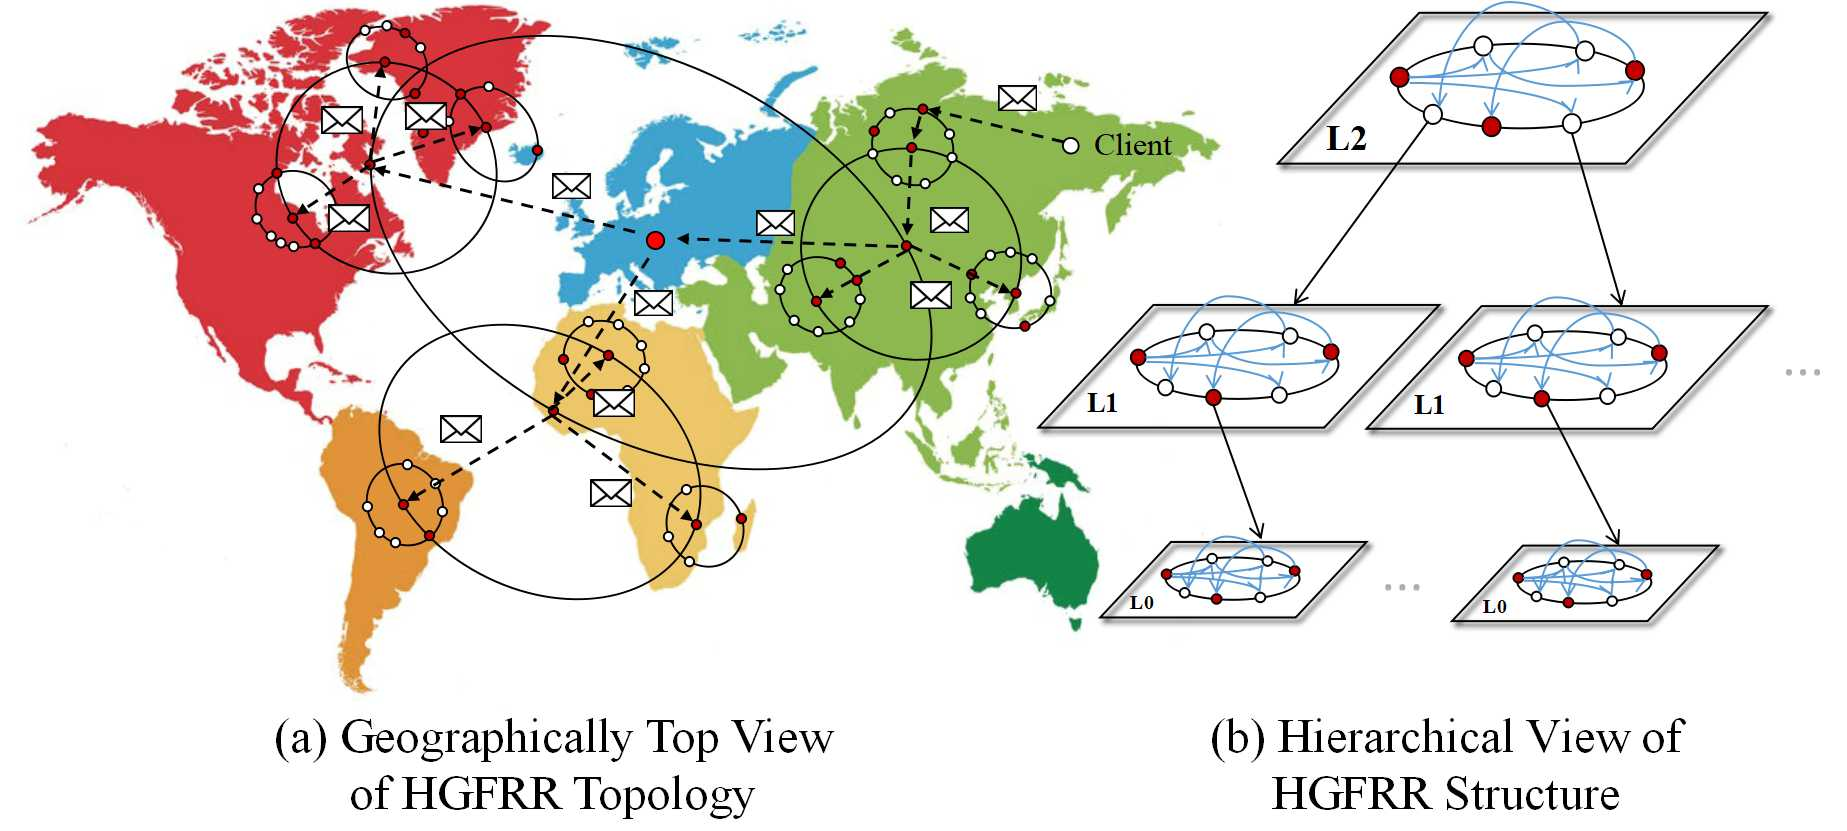
\includegraphics[width=0.5\textwidth]{figures/topo.jpg}
	\caption{Network Topology and Hierarchical Structure of HGFRR}
	\label{fig:topo}
\end{figure}

The network topology of HGFRR is basically a fractal-ring structure, where lower level rings reside on higher level rings (See Figure \ref{fig:topo}) in a recursive way. At the top level resides the largest ring where several sub-ring resides on while at the bottom level resides the smallest rings. The figure shows a network of 3 levels. Level 2 contains the largest ring. On the largest ring, there are three sub-rings of 2 levels. Level 1 contains the second largest rings and level 0 contains the smallest rings. The nodes in red are contact nodes of each ring. They are elected to be normal nodes of the upper level ring.

\subsubsection{Structure Formation} \label{formation}

When a new node wants to join the network, it will first send ping-messages to each of the contact nodes of the largest ring (at the top level). The new node will pick the contact node with the shorted response time to send a join-message. The contact node will then decide which sub-ring it should add this new node to, by sending the node information of contact nodes of each sub-ring back to the new node. Recursively, the new node will then choose the sub-ring which is optimal in terms of response time. And the contact node of the sub-ring will then introduce the new node to the sub-sub-ring. In the end, the contact node of a ring at the bottom level will then add the new node to the ring. If the number of node on the ring that the new node join to exceeds the threshold, then this ring will transform to a two-level ring (See Figure TODO), i.e. several groups of nodes on the large ring will form several rings. The transformation will be further elaborated in Section \cref{maintain}. After a new node joins the network, the contact node of this ring will broadcast within ring this node's information. The member nodes of this ring will then tell their information by sending welcome-messages to the new node.

The upper level rings are formed by contact node election. When a ring is first formed, the first member node of the ring will be the contact node of this ring. Each generation of contact nodes have their term of service. At the end of the term, one of the contact nodes will generate random IDs from all member node IDs. This election result will be dispersed within ring, and multi-casted to the contact nodes of the upper level ring and the lower level rings.

\begin{algorithm}
	\caption{Bootstrap}\label{euclid}
	\begin{algorithmic}[1]
		\Procedure{Node Join}{}
		\State $\var{response} \gets \var{queryDNSSeeds}()$
		\State $\var{contactNodeList} \gets \var{response.nodes}$
		\State $\var{level} \gets \var{response.topLevel}$
		\BState \emph{loop}:
		\If {$\var{level} = \var{0}$}
		\State $\textbf{break}$
		\Else
		\State $\var{optimalMetric} \gets \var{0}$
		\For {$\var{contactNode} : \var{contactNodeList}$}
		\State $\var{metric} \gets \var{testProximity}(\var{contactNode})$
		\If {$\var{metric} > \var{optimalMetric}$}
		\State $\var{optimalMetric} \gets \var{metric}$
		\State $\var{targetNode} \gets \var{contactNode}$
		\EndIf
		\EndFor
		\State $\var{response} \gets \var{queryNode}(\var{contactNode}, \var{level})$
		\State $\var{contactNodeList} \gets \var{response.nodes}$
		\State $\var{level} \gets \var{level}\var{-1}$
		\State \textbf{goto} \emph{loop}.
		\EndIf
		\State $/* \text{contact node of level 0 ring broadcast node-join}$
		\State $\text{\; * message withing the ring */}$
		\State $\var{this.}\var{nodeTable.insert}(\var{recvMsg.node})$
		\If {$\var{recvMsg.node.contactNode} = \var{true}$}
		\State $\var{contactNode} \gets \var{recvMsg.node}$
		\State $\var{contactNodeList.insert}(\var{contactNode})$
		\EndIf
		\EndProcedure
	\end{algorithmic}
\end{algorithm}

\subsubsection{Structure Maintenance} \label{maintain}

Each node on the bottom ring will send heart-beat messages to its successor and predecessor to check the aliveness of them. Once a node are not responding to the heart-beat message after the timeout value, the node will double check the liveness of this node with its, e.g. if A's predecessor B does not respond, A will check with the predecessor of B. If they agree that this node left the network (intentionally or accidentally), the information will be disseminated to the ring and this node will be officially removed from the network. If the missing node is the contact node, then the next generation of contact nodes will be elected. If the number of nodes on the ring is smaller than the lower limit, a transformation from right to left in Figure [TODO] will be performed.

\begin{algorithm}
	\caption{Maintenance}\label{euclid}
	\begin{algorithmic}[1]
		\State {\text{// This function will be called every \var{TIME\_INTERVAL}}}
		\Function{detect\_node\_left}{}
		\If{$\var{liveness\_check\_predecessor}() = \var{false}$}
		\State $\var{msg} \gets \var{constructNodeLeaveMSG}()$
		\State $\var{this.inRingBroadcast(msg)}$
		\EndIf
		\If{$\var{liveness\_check\_successor}() = \var{false}$}
		\State $\var{msg} \gets \var{constructNodeLeaveMSG}()$
		\State $\var{this.inRingBroadcast(msg)}$
		\EndIf
		\EndFunction
		\\
		\Function{liveness\_check\_predecessor}{}
		\State $\var{ret} = \var{sendHeartBeatMSG(this.predecessor)}$
		\If{$\var{ret.type} = \var{TIMEOUT}$}
		\State $\var{status} \gets \var{confirmWithPrePredecessor}()$
		\State \Return $\var{status}$
		\EndIf
		\EndFunction
		\\
		\Function{liveness\_check\_successor}{}
		\State $\var{ret} = \var{sendHeartBeatMSG(this.successor)}$
		\If{$\var{ret.type} = \var{TIMEOUT}$}
		\State $\var{status} \gets \var{confirmWithSucSuccessor}()$
		\State \Return $\var{status}$
		\EndIf
		\EndFunction
	\end{algorithmic}
\end{algorithm}

\subsection{Broadcast} \label{broadcast}

\textbf{Broadcast} is the process of disseminating a message from any node to the whole network. When a node wants to send a message to the whole network, it will first send broadcast-message to one of the contact nodes of the ring it resides on. Then the message will be routed to two directions: one direction is downwards, i.e. the contact node will broadcast the message in the ring and recursively in the sub-rings; the other direction is upwards, i.e. the contact node will send broadcast-message to one of the contact nodes of the upper level ring. Recursively, the broadcast-message will be received by one of the contact nodes of the largest ring. Then the contact node will broadcast recursively in the sub-rings. Till the bottom level, each node in the fractal ring will receive this message.

The k-ary distributed spanning tree method \cite{el2003efficient} is used to broadcast message in a ring. Details will be presented in the subsection. Based on this method, the time complexity of a broadcast operation will be $O(logN)$ and message complexity will be $(O(N))$, which are currently the best among related works.

\subsubsection{Broadcast Within-Ring Mechanism}

In-ring broadcast is based on the k-ary distributed spanning tree method. The basic idea is that the broadcast starter will first generate a random number $k$, and then a k-ary spanning tree can be formed in a distributed manner. Broadcast will then be triggered from the root to every node in the tree. The reason we choose to randomize the parameter k is that the network should be hidden from the attacker. If it keeps using the same parameter k, the routing pattern will be known easily by watching the network activities for a long time. The spanning tree are formed by using the broadcaster (which is numbered 0) as the root. Node 0 will connect to node $0+k^0$, $0+k^1$, $0+k^2$, and so on. Similarly, node 1 will connect to $1+k^0$, $1+k^1$, $1+k^2$, and so on. The pattern is: node $i$ will connect to $i+k^0$, $i+k^1$, $i+k^2$, and so on. The overall time complexity of this method will be $O(logN)$, where $N$ is the number of nodes in the ring.

[TODO] For example, Figure 4.3(a) shows a ring of 10 nodes numbered from 0 to 9. As the k-ary spanning tree algorithm states, when $k=2$: node 0 will connect to node 1, 2, 4, 8; node 1 will connect to node 3, 5, 9; node 2 will connect to node 6; node 3 will connect to node 7. After a spanning tree is formed (see Figure 4.3(b)), the message will be disseminated from node 0 down to every node in the spanning tree.

\begin{algorithm}
	\caption{Broadcast}\label{euclid}
	\begin{algorithmic}[1]
		\Function{broadcast}{\var{data}}
		\State $\var{level} \gets \var{0}$
		\State $\var{contactNode} \gets \var{selectFromContactNodes(level)}$
		\State $\var{message} \gets \var{wrapMessage(data)}$
		\State $\var{sendTo(contactNode, message)}$
		\EndFunction
		\\
		\Function{broadcast\_up}{\var{currentLevel, data}}
		\State $\var{level} \gets \var{currentLevel+1}$
		\State $\var{contactNode} \gets \var{selectFromContactNodes(level)}$
		\State $\var{message} \gets \var{wrapMessage(data)}$
		\State $\var{sendTo(contactNode, message)}$
		\EndFunction
		\\
		\Function{broadcast\_within\_ring}{\var{currentLevel, message, sentIDs, k}}
		\State $\var{endID} \gets \var{this.getNodeTableSize(currentLevel)}$
		\State $\var{i} \gets \var{0}$
		\State $\var{nodeOrder} \gets \var{message.nodeOrder}$
		\While {$\var{nodeOrder + pow(k, i)} < \var{endID}$}
		\State $\var{currentID = nodeOrder + pow(k, i)}$
			\If{$\var{pow(k, i) <= nodeOrder}$}
			\State $\var{i++}$
			\State $\textbf{continue}$
			\Else
			\State $\var{targetNodeID = NodeID + pow(k, i)}$
			\If{$\var{targetNodeID > endID}$}
			\State $\var{targetNodeID -= endID + 1}$
			\EndIf
			\State $\var{args=(targetNodeID, currentLevel)}$
			\State $\var{receiver} \gets (\var{this.getPeer(args)})$
			\State $\var{i++}$
			\State $\var{sendTo(receiver, message)}$
			\EndIf
		\EndWhile
		\EndFunction
	\end{algorithmic}
\end{algorithm}

\subsection{Security Consideration} \label{security}

Talk about the usage of Intel SGX[TODO].

To hide the existence of HGFRR contact nodes from outsiders, there are two mechanisms. First, fake messages are used to make the behavior of a contact node the same with that of a normal node. For a contact node, it will send messages of the same size to both one of the contact nodes and some of the past contact nodes in the upper level ring. For a normal node, it will send messages of the same size to both one of the contact nodes and some of its peers in the same level ring. When broadcasting messages withing the ring, the random parameter k will hide the relative orders of each node. Apart from broadcasting to its children in the constructed k-ary distributed spanning tree, each node will randomly choose a node to send fake message. All fake messages are of the same size of the real messages. Hackers may watch the packets sending out from a node and sending to the node for a long time. However, during one contact node service term, no difference can be discovered from the data collected. Second, contact nodes of a ring will be elected for every service term. One contact node of the last service term will generate random IDs by using Intel SGX's \texttt{sgx\_read\_rand ()} function \cite{costan2016intel}, and then broadcast the nomination result withing the ring. Due to both limited contact node service term period and the same behavior during one service term, outsider cannot differentiate contact nodes from normal nodes. HGFRR's network topology and structure are well hidden from the outsiders. Packet analysis is done by using WireShark and the evaluation result is discussed in Section [TODO].

\section{Proof and Analysis}
\subsection{Broadcast Message Complexity}

Consider a network of size $N$. All nodes in the network are geographically distributed evenly. 
In HGFRR, every $r$ nodes that are geographically near to each other will be gathered into a ring at the bottom level. 
If there are $c$ contact nodes in each ring at the bottom level, then the number of nodes elected to be the normal nodes at the second level will be: $$L(1) = \frac{cN}{r}$$ 
Then according to the protocol of HGFRR, the number of nodes elected to be the normal nodes at the next level will be the number of rings at the second level multiply with parameter $c$, which is: $$L(2) = \frac{c^2N}{r^2}$$ 
Recursively, the number of nodes $L(h)$ and the number of rings $R(h)$ at level $h$ will be: $$L(h) = \frac{c^hN}{r^h}, R(h)=\frac{c^hN}{r^{h+1}}$$ 
Let there be $T$ nodes in the top level (which are DNS seeds for a networked system), let $C = c/r$ be the contact node/normal node ratio at each ring, then the number of levels will be: $$l = log_{C}{\frac{T}{N}}$$
To broadcast a message from a node in any ring at the bottom level, the message will first be disseminated upwards until it reached the ring at the top level. The number of messages used to reach any contact nodes at the top level is: $$M_1(N)=1+l=1+log_{C}{\frac{T}{N}}$$
The number of messages used to broadcast from the top level rings recursively to all nodes in each ring at each level is: $$M_2(N)=\sum_{i=0}^{l} N\frac{c}{r}^i=N\frac{1-C^{l-1}}{1-C}$$
$$=\frac{CN-T}{C(1-C)}$$ Hence the message complexity of a broadcast operation is $O(N)$, which is better than current message complexity of both push Gossip ($O(NlogN)$) and push-pull Gossip ($O(NloglogN)$) \cite{jelasity2011gossip}.

\subsection{Broadcast Time Complexity}

Considering that the cost to transmit a data packet between two nodes in any two different continents is far larger than the cost to transmit between two nodes in the same city, let the cost of transmit data packets in different rings at level $h$ be $C(h)$, which is a mapping from levels to time cost constants. 
To broadcast a message from a node in any ring at the bottom level, the going-up path of the message to broadcast takes at most: $$T_1(N) = \sum_{i=1}^{l}C(i)$$
After the message reaches any of the contact nodes at the top level, the message starts to broadcast downwards recursively in each ring (in parallel) from the top level to the bottom level. The time it takes to touch each individual node at the bottom level is: $$T_2(N) = \sum_{i=0}^{l}C(i)\log_{k}{\frac{L(i)}{R(i)}}R(i)$$ $$= \sum_{i=0}^{l}C(i)\log_{k}{C^iN}$$
Hence the time complexity of a broadcast operation is $O(logN)$, which is also the complexity of the number of rounds in broadcast. Although the time complexity of Gossip algorithm is also $O(logN)$, in this case, if each node only connect to those nodes who have the smallest proximity in geographical locality, the total time complexity will be $O(N)$ \cite{kashyap2006efficient, kaune2008embracing}.

\subsection{Robustness}

In a blockchain system, individual machines are often under the control of a large number of heterogeneous users who may join or leave the network at any time. The dynamic of large-scale distributed system and link failure cause problems to the message dissemination. Since the dissemination of membership information and transactions require to reach all nodes, even the consensus protocol requires the message to reach at least a half (PoW, PoS, DPoS, Ripple) or two thirds (BFT, PBFT, Tendermint, Algorand BA*) \cite{zheng2016blockchain}, the P2P network under a blockchain system should try the best to reach as many nodes as possible. Under dynamic node joining/leaving and link failure, the network should be robust enough to cover as many as possible the remaining working nodes.
To analyze the robustness of HGFRR, we define reliability metric to be the ratio of covered nodes and remaining nodes. Let the probability of node failure be $p$, therefore, the number of nodes cannot be reached is: $$F(N)=\sum_{i=1}^{l} \sum_{j=i+1}^{l}(1-p)^jp^cR(i)r^{i}$$
%=\sum_{i=1}^{l} p^c\frac{c^iN}{r}=p^c\frac{Nc(1-c^l)}{r(1-c)}
Thus the reliability of HGFRR will be: $$Reliability = \frac{N-F(N)}{(1-p)N}$$
%=\frac{1-p^c\frac{c(1-c^l)}{r(1-c)}}{1-p}$$ 
%$$\frac{1}{1-p}-\frac{p^cC(1-c^l)}{(1-p)(1-c)}
In the context of blockchain systems, a 7-level HGFRR will reach 1/2 of all nodes on broadcasting a message if the node failure rate is less than 13.8\%, and will reach 2/3 of all nodes if the failure rate is less than 13.3\%. In the evaluation, we set the fault rate of all nodes to be from 10\% to 70\%, the reliability of HGFRR can reach the same level with Gossip. And we found that in blockchain system context, Gossip is overly strong in terms of robustness. As the consensus protocol of a blockchain system only need responses from a half or two thirds of all nodes to be honest, we could trade fault-tolerance off to gain efficiency.

\section{Implementation Details}
We have implemented \xxx in C++. An \xxx application running on a server mainly includes three components, a \texttt{NodeTable}, a \texttt{PeerManager}, and a \texttt{Discoverer}. The \texttt{Discoverer} is responsible for bootstrapping node. The \texttt{NodeTable} stores peer information at each level and maintains the network structure. The \texttt{PeerManager} deal with incoming messages and is responsible for broadcasting messages.

The source code of \xxx will be available at \texttt{github} \texttt{.com/hku-systems/hgfrr}.

\section{Evaluation}
This is the evaluation. \\

how we evaluated hgfrr.

\subsection{Evaluation Setup}

talk about how we set up the evaluation

\subsection{Ease of Use}

use kad+gossip to substitute eth

\subsection{Performance Improvements}

talk about the performance improvement in terms of convergence time, message complexity.

\subsubsection{Broadcast}

broadcast performance

\subsubsection{Robustness and Scalability}

fault-tolerance and scalability of broadcast

\subsubsection{Contact Node Election}

performance of contact node election

\subsubsection{Node Join and Leave}

performance of node join and leave, which may lead to structure change

\subsection{Security Evaluation}

wireshark analysis to show the anonymity of contact nodes

\begin{table} \label{packet}
	\begin{tabular}{l*{6}{c}r}
		Node Type & $\sim17 KB$ & $\sim200 B$ & $<150 B$ \\
		\hline		
		Normal node in one term & 33.10\%	& 58.60\% & 5.90\% \\
		Contact node in one term & 34.00\%	& 61.20\% &4.50\%  \\
		Node at all time  & 33.70\%	& 60.90\% &4.60\%  \\
	\end{tabular}
	\caption{Send-Packet Analysis of Node in HGFRR}
	\vspace{2mm}
	\begin{tabular}{l*{6}{c}r}
		Node Type & $\sim17 KB$ & $\sim200 B$ & $<150 B$ \\
		\hline		
		Normal node in one term & 35.50\% & 58.60\% & 5.60\% \\
		Contact node in one term & 34.40\% & 59.20\% & 4.70\%  \\
		Node at all time  & 34.60\% & 59.10\% & 5.10\%  \\
	\end{tabular}
	\caption{Receive-Packet Analysis of Node in HGFRR}
\end{table}

\section{Related Work}
This is the related work. \\

\noindent
\textbf{P2P Network in Ethereum} Talk about kademlia+gossip in ethereum.\\
\noindent
\textbf{Broadcast in DHT} Talk about a work working on broadcast in dht.
\\
more to be added and compared.

\section{Conclusion}
This paper identifies the problem of using Gossip in the P2P network layer of a blockchain system, which to some extent already became the bottleneck of further improving the transaction rate. Though tremendous work has been proposed in consensus layer to improve transaction rate, few work addressed the problem from the P2P network layer. \xxx makes use of the recursive structure to broadcast messages so that messages redundancy could be reduced to the lowest. \xxx also take the geographical locality of each node into consideration to further improve the efficiency of a broadcast operation. \xxx is robust even in a dynamic network environment and is hidden from outsiders. Although \xxx is not as robust as Gossip, it is evaluated and analyzed that the robustness of \xxx is sufficient in blockchain system context. By trading robustness, \xxx improves the throughput of blockchain systems by increasing broadcast efficiency. In the future, the transaction rate of the blockchain systems can be improved further in a low bandwidth-consumption or crowded network.

\section{Acknowledgments}

A polite author always includes acknowledgments.  Thank everyone,
especially those who funded the work. 

%%%%%%%%%%%%%%%%%%%%%% End %%%%%%%%%%%%%%%%%%%%%%%%%

\section{ATC Template For Reference}

{\tt \small
\begin{verbatim}
int wrap_fact(ClientData clientData,
              Tcl_Interp *interp,
              int argc, char *argv[]) {
    int result;
    int arg0;
    if (argc != 2) {
        interp->result = "wrong # args";
        return TCL_ERROR;
    }
    arg0 = atoi(argv[1]);
    result = fact(arg0);
    sprintf(interp->result,"%d",result);
    return TCL_OK;
}
\end{verbatim}
}

Now we're going to cite somebody.  Watch for the cite tag.
Here it comes~\cite{stoica2001chord}.  The tilde character (\~{})
in the source means a non-breaking space.  This way, your reference will
always be attached to the word that preceded it, instead of going to the
next line.

More fascinating text. Features\endnote{Remember to use endnotes, not footnotes!} galore, plethora of promises.\\

\section{This Section has SubSections}
\subsection{First SubSection}

Here's a typical figure reference.  The figure is centered at the
top of the column.  It's scaled.  It's explicitly placed.  You'll
have to tweak the numbers to get what you want.\\

% you can also use the wonderful epsfig package...
\begin{figure}[t]
\begin{center}
\begin{picture}(300,150)(0,200)
\put(-15,-30){\special{psfile = fig1.ps hscale = 50 vscale = 50}}
\end{picture}\\
\end{center}
\caption{Wonderful Flowchart}
\end{figure}

This text came after the figure, so we'll casually refer to Figure 1
as we go on our merry way.

\subsection{New Subsection}

It can get tricky typesetting Tcl and C code in LaTeX because they share
a lot of mystical feelings about certain magic characters.  You
will have to do a lot of escaping to typeset curly braces and percent
signs, for example, like this:
``The {\tt \%module} directive
sets the name of the initialization function.  This is optional, but is
recommended if building a Tcl 7.5 module.
Everything inside the {\tt \%\{, \%\}}
block is copied directly into the output. allowing the inclusion of
header files and additional C code." \\

Sometimes you want to really call attention to a piece of text.  You
can center it in the column like this:
\begin{center}
{\tt \_1008e614\_Vector\_p}
\end{center}
and people will really notice it.\\

\noindent
The noindent at the start of this paragraph makes it clear that it's
a continuation of the preceding text, not a new para in its own right.


Now this is an ingenious way to get a forced space.
{\tt Real~$*$} and {\tt double~$*$} are equivalent. 

Now here is another way to call attention to a line of code, but instead
of centering it, we noindent and bold it.\\

\noindent
{\bf \tt size\_t : fread ptr size nobj stream } \\

And here we have made an indented para like a definition tag (dt)
in HTML.  You don't need a surrounding list macro pair.
\begin{itemize}
\item[]  {\tt fread} reads from {\tt stream} into the array {\tt ptr} at
most {\tt nobj} objects of size {\tt size}.   {\tt fread} returns
the number of objects read. 
\end{itemize}
This concludes the definitions tag.

{\normalsize \bibliographystyle{acm}
\bibliography{./main}}

\theendnotes

\end{document}